\documentclass{article}
\usepackage{tikz, comment}
\usepackage{pifont}
\usepackage{fontspec}
\usetikzlibrary{arrows, decorations.markings, decorations.pathreplacing}
\begin{comment}
:Title: Not defined yet
:Tags: approximation by differentials;equation of a line;inverse variation, inverse proportion , inversely proportional ;absolute value rules;focal radius 
:Prob: 0.4121;0.401;0.3988;0.3939;0.387
:Author: Prof.Hu Ji-shan, HKUST
:Slug: No name yet

Description Here.........
\end{comment}
\begin{document}\centering

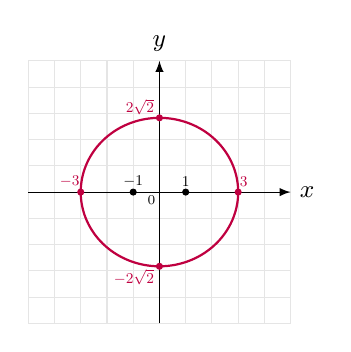
\begin{tikzpicture}[>=latex,xscale=.5/1.5, yscale=.5/1.5][font=\sf\small]

\draw[xstep=1cm,ystep=1cm,color=gray!20] (-5, -5) grid (5, 5);

\draw[->] ({-5}, 0) -- ({5}, 0)node[right] {\small $x$};
\draw[->] (0, {-5}) -- (0, {5})node[above] {\small $y$};

\clip[] (-5, -5) rectangle (5, 5);

\draw[purple, thick, samples=100, smooth, domain=0:2*pi, variable=\t]
plot ({sqrt(9)*cos(\t r)}, {sqrt(8)*sin(\t r)});

%\node[purple, xshift=-50, yshift=20, scale=0.6] at (0,0) {$y^2+2y+12x+25 = 0$};

\draw[black, fill, xscale=1.5, yscale=1.5] ({sqrt(9-8)/1.5}, {0/1.5}) circle(0.075)node[above, xshift=0, yshift=0, scale=0.6] {$1$};
\draw[black, fill, xscale=1.5, yscale=1.5] ({-sqrt(9-8)/1.5}, {0/1.5}) circle(0.075)node[above, xshift=0, yshift=0, scale=0.6] {$-1$};

\draw[purple, fill, xscale=1.5, yscale=1.5] ({sqrt(9)/1.5}, {0/1.5}) circle(0.075)node[above, xshift=2, yshift=0, scale=0.6] {$3$};
\draw[purple, fill, xscale=1.5, yscale=1.5] ({-sqrt(9)/1.5}, {0/1.5}) circle(0.075)node[above, xshift=-4, yshift=0, scale=0.6] {$-3$};

\draw[purple, fill, xscale=1.5, yscale=1.5] ({0/1.5}, {sqrt(8)/1.5}) circle(0.075)node[left, xshift=0, yshift=4, scale=0.6] {$2\sqrt 2$};
\draw[purple, fill, xscale=1.5, yscale=1.5] ({0/1.5}, {-sqrt(8)/1.5}) circle(0.075)node[left, xshift=0, yshift=-4, scale=0.6] {$-2\sqrt 2$};

\node[scale=0.7] at (-0.2*1.5, -0.2*1.5) {\scriptsize$0$};

\end{tikzpicture}
\end{document}